% On découpe ce document complexe en plusieurs sous-fichiers séparés.
% Cela permettra notamment de réarranger les transparents facilement
% lors de l'élaboration du document.

% La définition de la classe beamer avec tous les styles afférents
%%%%%%%%%%%%%%%%%%%%%%%%%%%%%%%%%%%%%%%%%
% Beamer Presentation
% LaTeX Template
% Version 1.0 (10/11/12)
%
% This template has been downloaded from:
% http://www.LaTeXTemplates.com
%
% License:
% CC BY-NC-SA 3.0 (http://creativecommons.org/licenses/by-nc-sa/3.0/)
%
%%%%%%%%%%%%%%%%%%%%%%%%%%%%%%%%%%%%%%%%%

%----------------------------------------------------------------------------------------
%	PACKAGES AND THEMES
%----------------------------------------------------------------------------------------

\RequirePackage{currfile}

\documentclass[aspectratio=43, landscape]{beamer}


\mode<presentation> {

\RequirePackage{appendixnumberbeamer}% Don't number appendix frames.


% The Beamer class comes with a number of default slide themes
% which change the colors and layouts of slides. Below this is a list
% of all the themes, uncomment each in turn to see what they look like.

%\usetheme{default}
%\usetheme{AnnArbor}
%\usetheme{Antibes}
%\usetheme{Bergen}
%\usetheme{Berkeley}
%\usetheme{Berlin}
%\usetheme{Boadilla}
%\usetheme{CambridgeUS}
%\usetheme{Copenhagen}
\usetheme{Darmstadt}
%\usetheme{Dresden}
%\usetheme{Frankfurt}
%\usetheme{Goettingen}
%\usetheme{Hannover}
%\usetheme{Ilmenau}
%\usetheme{JuanLesPins}
%\usetheme{Luebeck}
%\usetheme{Madrid}
%\usetheme{Malmoe}
%\usetheme{Marburg}
%\usetheme{Montpellier}
%\usetheme{PaloAlto}
%\usetheme{Pittsburgh}
%\usetheme{Rochester}
%\usetheme{Singapore}
%\usetheme{Szeged}
%\usetheme{Warsaw}

% As well as themes, the Beamer class has a number of color themes
% for any slide theme. Uncomment each of these in turn to see how it
% changes the colors of your current slide theme.

%\usecolortheme{albatross}
%\usecolortheme{beaver}
%\usecolortheme{beetle}
%\usecolortheme{crane}
%\usecolortheme{dolphin}
%\usecolortheme{dove}
%\usecolortheme{fly}
%\usecolortheme{lily}
%\usecolortheme{orchid}
%\usecolortheme{rose}
%\usecolortheme{seagull}
%\usecolortheme{seahorse}
\usecolortheme{whale}
%\usecolortheme{wolverine}

%\setbeamertemplate{footline} % To remove the footer line in all slides uncomment this line
%\setbeamertemplate{footline}[frame number] % To replace the footer line in all slides with a simple slide count uncomment this line

%\setbeamertemplate{navigation symbols}{} % To remove the navigation symbols from the bottom of all slides uncomment this line

\setbeamercovered{transparent} % Fait apparaître les animations en grisé (utile pour la conception, mais peut être commenté lors de la remise du document final)

% Pour utiliser une police à empattements partout
\usefonttheme{serif}

% Pour rajouter la numérotation des frames dans les pieds de page
\newcommand*\oldmacro{}%
\let\oldmacro\insertshorttitle%
%\renewcommand*\insertshorttitle{%
%  \oldmacro\hfill%
%  \insertframenumber\,/\,\inserttotalframenumber}
%


\makeatletter
\setbeamertemplate{footline}
{
    \leavevmode%
    \hbox{%
        \begin{beamercolorbox}[wd=.333333\paperwidth,ht=2.25ex,dp=1ex,center]{author in head/foot}%
            \usebeamerfont{author in head/foot}\insertshortauthor
        \end{beamercolorbox}%
        \begin{beamercolorbox}[wd=.333333\paperwidth,ht=2.25ex,dp=1ex,center]{title in head/foot}%
            \usebeamerfont{title in head/foot}\insertshorttitle
        \end{beamercolorbox}%
        \begin{beamercolorbox}[wd=.333333\paperwidth,ht=2.25ex,dp=1ex,right]{date in head/foot}%
            \usebeamerfont{date in head/foot}\insertshortdate{}\hspace*{2em}
            \insertframenumber{} / \inserttotalframenumber\hspace*{2ex}
        \end{beamercolorbox}}%
        \vskip0pt%
    }
    \makeatother

    \AtBeginSection[]
    {
    \begin{frame}{Plan de l'exposé}
      \tableofcontents[currentsection]
    \end{frame}
    }

}

% Pour ne pas numéroter certaines diapos
\newcommand{\backupbegin}{
  \newcounter{framenumberappendix}
  \setcounter{framenumberappendix}{\value{framenumber}}
  \setbeamertemplate{footline}{}
}
\newcommand{\backupend}{
  \addtocounter{framenumberappendix}{-\value{framenumber}}
  \addtocounter{framenumber}{\value{framenumberappendix}}
  \setbeamertemplate{footline}{
    \vspace{-1cm}\small{\insertframenumber/\inserttotalframenumber}
  }
}

\usepackage{graphicx} % Allows including images
\usepackage{booktabs} % Allows the use of \toprule, \midrule and \bottomrule in tables

% Pour numéroter les figures
\setbeamertemplate{caption}[numbered]


% Les autres packages utiles  notamment pour le français, les accents ou Python
\usepackage{natbib}         % Pour la bibliographie
\usepackage{url}            % Pour citer les adresses web
\usepackage[T1]{fontenc}    % Encodage des accents
\usepackage[utf8]{inputenc} % Lui aussi
\usepackage[french]{babel} % Pour la traduction française
\usepackage{numprint}       % Histoire que les chiffres soient bien

\usepackage{amsmath}        % La base pour les maths
\usepackage{mathrsfs}       % Quelques symboles supplémentaires
\usepackage{amssymb}        % encore des symboles.
\usepackage{amsfonts}       % Des fontes, eg pour \mathbb.

\usepackage{cancel}
\usepackage{listings}
\usepackage{xcolor}  % ajout de ce package pour pouvoir définir et utiliser des couleurs

% Définition des couleurs
\definecolor{dkgreen}{rgb}{0,0.6,0}
\definecolor{mauve}{rgb}{0.58,0,0.82}
\definecolor{gray}{rgb}{0.5,0.5,0.5}


%\usepackage[svgnames]{xcolor} % De la couleur

%%% Si jamais vous voulez changer de police: décommentez les trois 
%\usepackage{tgpagella}
%\usepackage{tgadventor}
%\usepackage{inconsolata}

%%% Pour L'utilisation de Python
\usepackage{minted}
\usemintedstyle{friendly}

\usepackage{graphicx} % inclusion des graphiques
\usepackage{wrapfig}  % Dessins dans le texte.

\usepackage{tikz}     % Un package pour les dessins (utilisé pour l'environnement {code})
\usepackage[framemethod=TikZ]{mdframed}

% Les macros et raccourcis personnels
% Ce fichier contient toutes les macros que vous pouvez avoir envie de définir 
% si vous les utilisez plusieurs fois dans le document.

\PassOptionsToPackage{svgnames}{color}

% Un environnement pour bien présenter le code informatique
\newenvironment{code}{%
\begin{mdframed}[linecolor=green,innerrightmargin=30pt,innerleftmargin=30pt,
backgroundcolor=black!5,
skipabove=10pt,skipbelow=10pt,roundcorner=5pt,
splitbottomskip=6pt,splittopskip=12pt]
}{%
\end{mdframed}
}

% Un raccourci pour composer les unités correctement (en droit)
% Exemple: $v = 10\U{m.s^{-1}}$
\newcommand{\U}[1]{~\mathrm{#1}}

% Les guillemets \ofg{par exemple}
\newcommand{\ofg}[1]{\og{}#1\fg{}}

% Le d des dérivées doit être droit: \frac{\dd x}{\dd t}
\newcommand{\dd}{\text{d}}

% La dérivée temporelle, tellement courante en physique, avec les d droits
\newcommand{\ddt}[1]{\frac{\dd #1}{\dd t}}

% Des parenthèses, crochets et accolades qui s'adaptent automatiquement à la 
% taille de ce qu'il y a dedans
\newcommand{\pa}[1]{\left(#1\right)}
\newcommand{\pac}[1]{\left[#1\right]}
\newcommand{\paa}[1]{\left\{#1\right\}}

% Un raccourci pour écrire une constante
\newcommand{\cte}{\text{C}^{\text{te}}}

% Pour faire des indices en mode texte (comme les énergie potentielles)
\newcommand{\e}[1]{_{\text{#1}}}

% Le produit vectoriel a un nom bizarre:
\newcommand{\vectoriel}{\wedge}


% On définit le titre et l'auteur du document

% L'argument optionnel (entre crochets) donne le titre qui sera mis sur chaque slide
\title[TIPE Ville]{TIPE: Modélisation et Prévision du
risque de cambriolage en ville}
\author[M. MUNIER]{MUNIER Maxime - Candidat 38530} % Votre nom (pour cette année) ou numéro (pour le concours)
% L'épreuve (car on n'a pas le droit de signaler sa provenance à un concours) 
% (là encore, l'argument optionnel apparaît sur chaque slide)
\institute[TIPE]{Épreuve de TIPE}
\date{Session 2023}

% Optionnel : personnalisation de l'affichage du code Python
\lstset{
  language=Python,
  basicstyle=\ttfamily\small,
  numbers=left,
  numberstyle=\tiny\color{gray},
  commentstyle=\color{dkgreen},
  stringstyle=\color{mauve},
  breaklines=true,
  breakatwhitespace=true,
  tabsize=3
}

% On démarre le document proprement dit
\begin{document}

% La page de titre et la table des matières
% Rien d'autre à faire qu'afficher le titre
\begin{frame}
  \titlepage
\end{frame}


% La table des matières utilise ce que vous donnez aux commandes \section et
% \subsection tout au long de la présentation.
\begin{frame}
  \frametitle{Plan de l'exposé}
  \tableofcontents
\end{frame}


% La première grande partie: introduction du sujet
% Titre de la premiere partie
\section[Théorie]{Présentation théorique des Processus de Hawkes}

%%%%%%%%%%%%%%%%%%%%%%%%%%%%%%%%%%%%%%%%%%%%%%%%
% Première diapo
%%%%%%%%%%%%%%%%%%%%%%%%%%%%%%%%%%%%%%%%%%%%%%%%
\begin{frame}
	\frametitle{Présentation théorique des Processus de Hawkes}
	\framesubtitle{Définition d'un processus de Hawkes à une dimension}

	\begin{block}{Processus de Hawkes}
		Un processus de Hawkes à une dimension est un processus stochastique ponctuel qui modélise une série d'événements unidimensionnels dans le temps. Il est défini par sa fonction d'intensité conditionnelle, qui décrit la probabilité d'occurrence d'un événement à un instant donné, en fonction de l'historique des événements précédents.
	\end{block}

\end{frame}

\begin{frame}
    \frametitle{Présentation théorique des Processus de Hawkes}
    \framesubtitle{Application aux cambriolages}

    \begin{block}{Pourquoi choisir les processus de Hawkes pour modéliser les risques de cambriolages en ville?}

        \begin{itemize}
            \item Modélisation de la dépendance temporelle
            \item Effet auto-excitateur
            \item Adaptation aux caractéristiques locales
            \item Prise en compte des événements antérieurs
            \item Flexibilité et adaptation aux données
            \item Applications pratiques
        \end{itemize}
    \end{block}
\end{frame}


\begin{frame}
    \frametitle{Présentation théorique des Processus de Hawkes}
    \framesubtitle{Définition d'un processus de Hawkes à une dimension}

    \begin{block}{Représentation mathématique}
        \[ N(t) = \sum_i \delta(t - t_i) \]

        \begin{itemize}
            \item $N(t)$ : nombre d'événements qui se sont produits jusqu'à l'instant $t$
            \item $t_i$ : instants auxquels les événements se sont produits
            \item $\delta(t - t_i)$ : fonction delta de Dirac qui vaut 1 si $t = t_i$ et 0 sinon.
        \end{itemize}
    \end{block}

\end{frame}


\begin{frame}

\begin{alertblock}{Objectif}
		L'objet de notre étude est de déterminer le nombre de cambriolages $N(t)$ au cours d'une période $[0, T]$, où $N(t)$ est un processus de Hawkes d'intensité $\lambda(t)$, $t \geq 0$.
	\end{alertblock}

\begin{block}{Exemple}
\begin{figure}[h!]
\centering
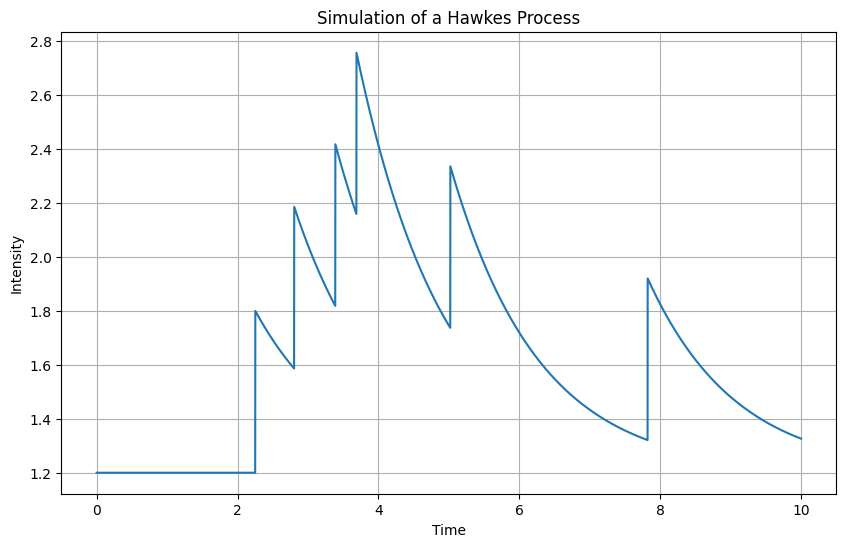
\includegraphics[width=0.6\linewidth]{figures/hawkes_process.png}
\label{fig:hawkes_process}
\end{figure}
\end{block}
\end{frame}


\begin{frame}
    \frametitle{Présentation théorique des Processus de Hawkes}
    \framesubtitle{Interprétation de la forme du modèle}

    \begin{block}{Représentation mathématique}
        \[ \lambda(t) = \lambda_0 + \sum_i \alpha_i \cdot e^{-\beta_i \cdot (t - t_i)} \]

        \begin{itemize}
            \item $\lambda(t)$ : fonction d'intensité conditionnelle à l'instant $t$
            \item $\lambda_0$ : taux de base (taux d'événements en l'absence d'influence des événements passés)
            \item $\alpha_i$ : coefficient d'excitation correspondant à l'événement $i$
            \item $\beta_i$ : coefficient de décroissance correspondant à l'événement $i$
            \item $t_i$ : temps de l'événement $i$
        \end{itemize}
    \end{block}
\end{frame}


\begin{frame}
    \frametitle{Présentation théorique des Processus de Hawkes}
    \framesubtitle{Interprétation des paramètres}

    \begin{block}{Influence du paramètre $\lambda_0$ }
    \[ \lambda(t) = \lambda_0 + \sum_i \alpha_i \cdot e^{-\beta_i \cdot (t - t_i)} \]

    \begin{itemize}
            \item $\lambda(t)$ : fonction d'intensité conditionnelle à l'instant $t$
            \item $\alpha_i$ : coefficient d'excitation correspondant à l'événement $i$ fixé à 0.6
            \item $\beta_i$ : coefficient de décroissance correspondant à l'événement $i$ fixé à 0.8
            \item $t_i$ : temps de l'événement $i$
        \end{itemize}

    \end{block}
\end{frame}
\begin{frame}
    \begin{block}{$\lambda_0$ = 0.01}
    \begin{figure}[h]
        \centering
        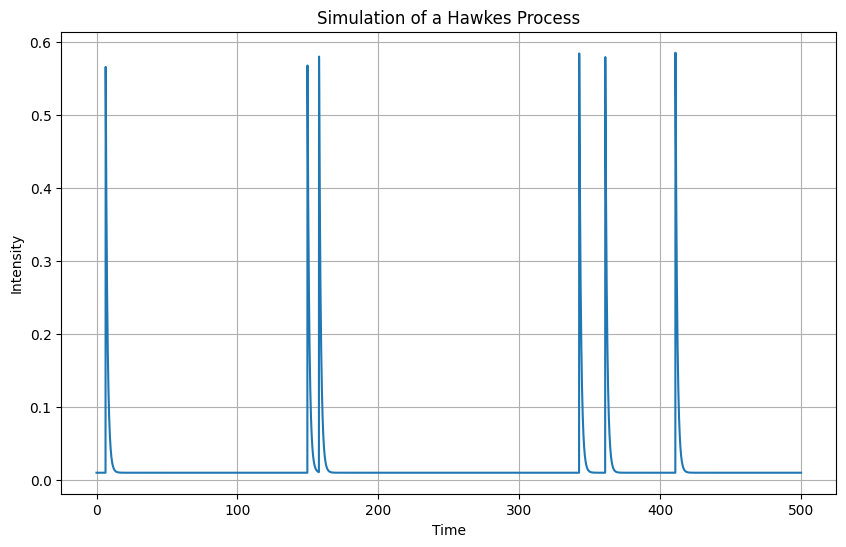
\includegraphics[width=0.6\linewidth]{figures/lamba1.png}
    \end{figure}
    \end{block}
\end{frame}

\begin{frame}
    \begin{block}{$\lambda_0$ = 0.1}
    \begin{figure}[h]
        \centering
        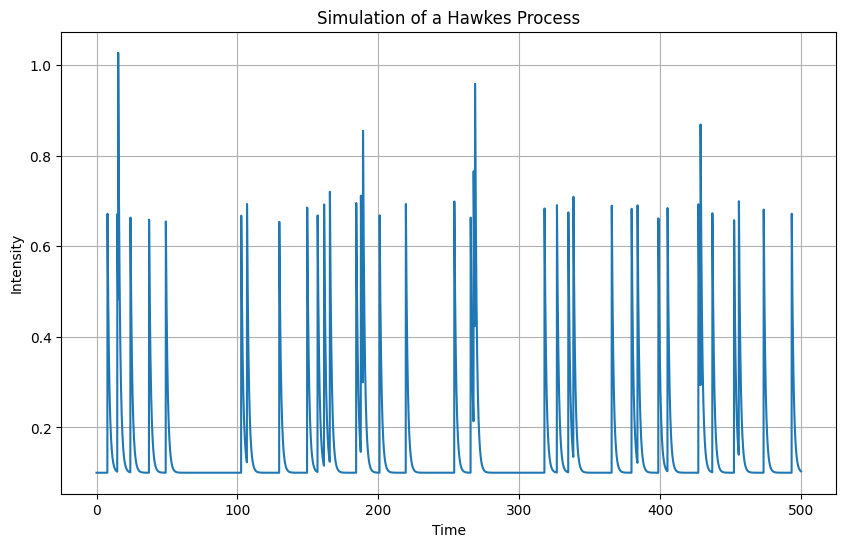
\includegraphics[width=0.6\linewidth]{figures/lambda2.png}
    \end{figure}
    \end{block}
\end{frame}

\begin{frame}
    \begin{block}{$\lambda_0$ = 1}
    \begin{figure}[h]
        \centering
        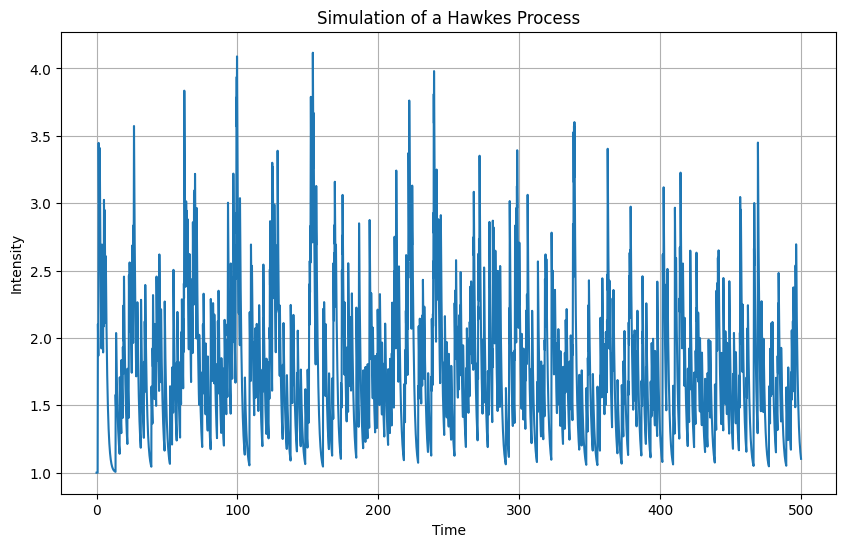
\includegraphics[width=0.6\linewidth]{figures/lambda3.png}
    \end{figure}
    \end{block}
\end{frame}

\begin{frame}
    \frametitle{Présentation théorique des Processus de Hawkes}
    \framesubtitle{Interprétation des paramètres}

    \begin{block}{Influence du paramètre $\alpha$ }
    \[ \lambda(t) = \lambda_0 + \sum_i \alpha_i \cdot e^{-\beta_i \cdot (t - t_i)} \]

    \begin{itemize}
            \item $\lambda(t)$ : fonction d'intensité conditionnelle à l'instant $t$
            \item $\lambda_0$ : taux de base (taux d'événements en l'absence d'influence des événements passés) fixé à 0.1
            \item $\beta_i$ : coefficient de décroissance correspondant à l'événement $i$ fixé à 1.2
            \item $t_i$ : temps de l'événement $i$
        \end{itemize}

    \end{block}
\end{frame}
\begin{frame}
    \begin{block}{$\alpha$ = 0.01}
    \begin{figure}[h]
        \centering
        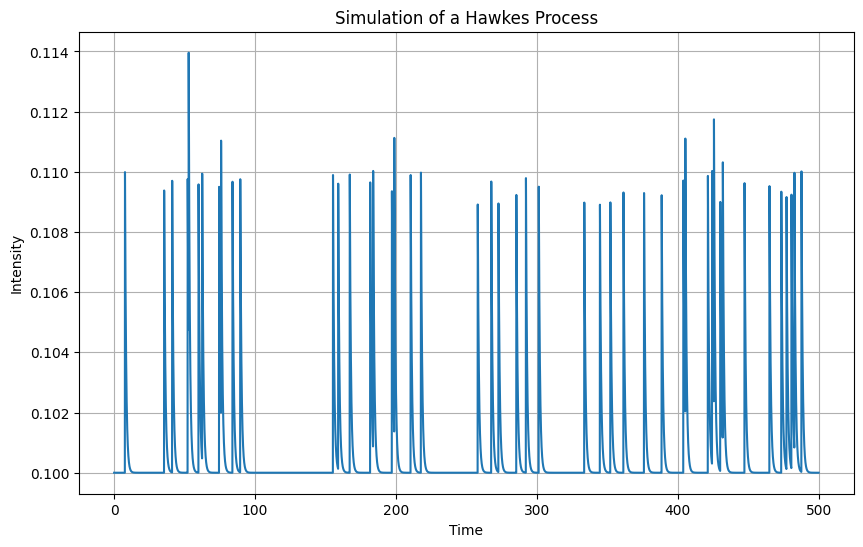
\includegraphics[width=0.6\linewidth]{figures/alpha1.png}
    \end{figure}
    \end{block}
\end{frame}

\begin{frame}
    \begin{block}{$\alpha$ = 0.1}
    \begin{figure}[h]
        \centering
        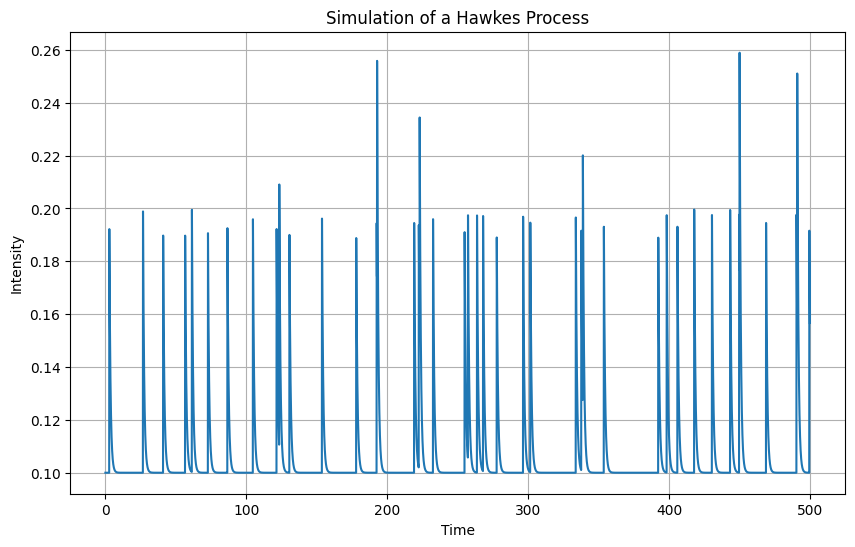
\includegraphics[width=0.6\linewidth]{figures/alpha2.png}
    \end{figure}
    \end{block}
\end{frame}

\begin{frame}
    \begin{block}{$\alpha$ = 1}
    \begin{figure}[h]
        \centering
        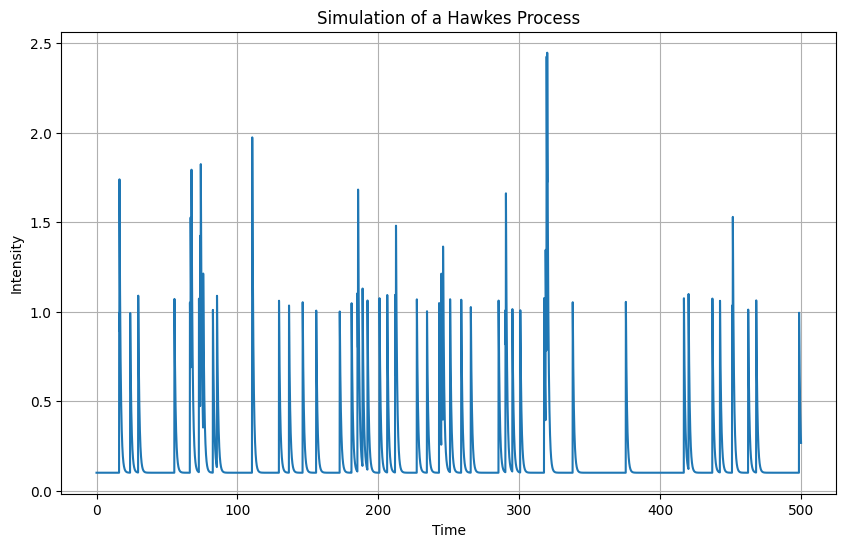
\includegraphics[width=0.6\linewidth]{figures/alpha3.png}
    \end{figure}
    \end{block}
\end{frame}

\begin{frame}
    \frametitle{Présentation théorique des Processus de Hawkes}
    \framesubtitle{Interprétation des paramètres}

    \begin{block}{Influence du paramètre $\beta$ }
    \[ \lambda(t) = \lambda_0 + \sum_i \alpha_i \cdot e^{-\beta_i \cdot (t - t_i)} \]

    \begin{itemize}
            \item $\lambda(t)$ : fonction d'intensité conditionnelle à l'instant $t$
            \item $\lambda_0$ : taux de base (taux d'événements en l'absence d'influence des événements passés) fixé à 0.1
            \item $\alpha_i$ : coefficient d'excitation correspondant à l'événement $i$ fixé à 0.6
            \item $t_i$ : temps de l'événement $i$
        \end{itemize}

    \end{block}
\end{frame}
\begin{frame}
    \begin{block}{$\beta$ = 0.05}
    \begin{figure}[h]
        \centering
        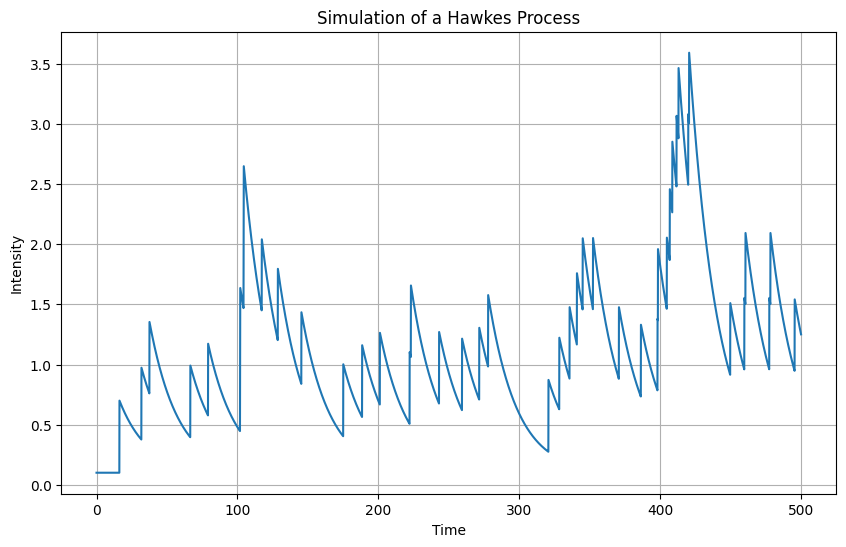
\includegraphics[width=0.6\linewidth]{figures/beta1.png}
    \end{figure}
    \end{block}
\end{frame}

\begin{frame}
    \begin{block}{$\beta$ = 0.5}
    \begin{figure}[h]
        \centering
        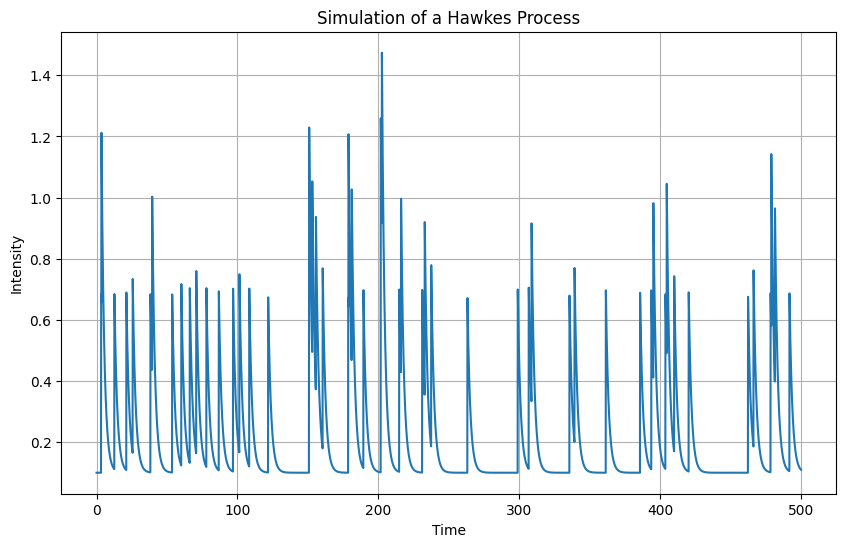
\includegraphics[width=0.6\linewidth]{figures/beta2.png}
    \end{figure}
    \end{block}
\end{frame}

\begin{frame}
    \begin{block}{$\beta$ = 5}
    \begin{figure}[h]
        \centering
        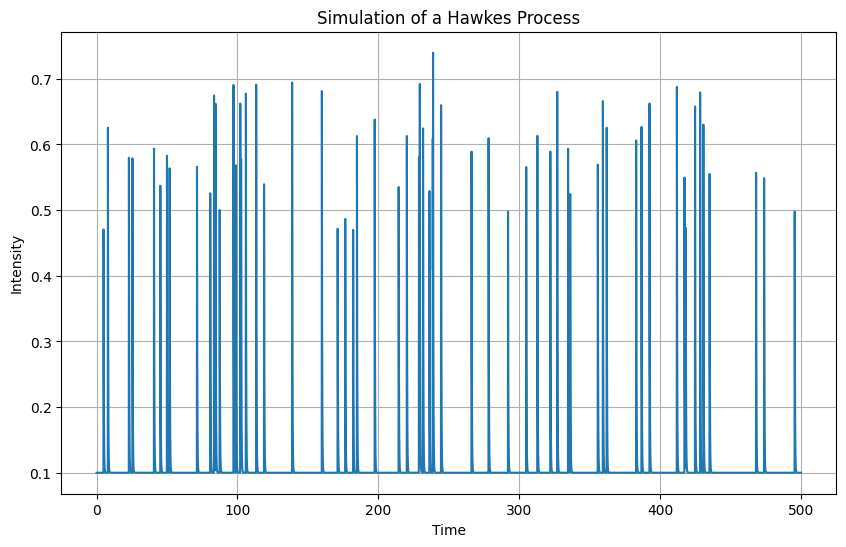
\includegraphics[width=0.6\linewidth]{figures/beta3.png}
    \end{figure}
    \end{block}
\end{frame}

\begin{frame}
    \frametitle{Présentation théorique des Processus de Hawkes}
    \framesubtitle{Simulation d'un processus de Hawkes}

    \begin{block}{Algorithme d'Ogata}
        L'algorithme d'Ogata (1981) génère des temps de survenance suivant un processus de Hawkes sur un intervalle de temps [0,T] en utilisant les paramètres $\lambda_0$, $\alpha$ et $\beta$, ainsi que la fonction d'intensité $\lambda$ qui dépend de ces trois paramètres.
    \end{block}
\end{frame}


\begin{frame}
    \frametitle{Présentation théorique des Processus de Hawkes}
    \framesubtitle{Estimation des paramètres}

    \begin{block}{Méthode du maximum de vraissemblance}
    La méthode du maximum de log-vraisemblance (ML pour Maximum Likelihood) est une technique statistique couramment utilisée pour estimer les paramètres d'un modèle statistique. L'idée est de trouver les paramètres du modèle qui maximisent la fonction de log-vraisemblance.

    \end{block}
\end{frame}

\begin{frame}
    \frametitle{Présentation théorique des Processus de Hawkes}
    \framesubtitle{Estimation des paramètres}
        \begin{figure}[h]
            \centering
            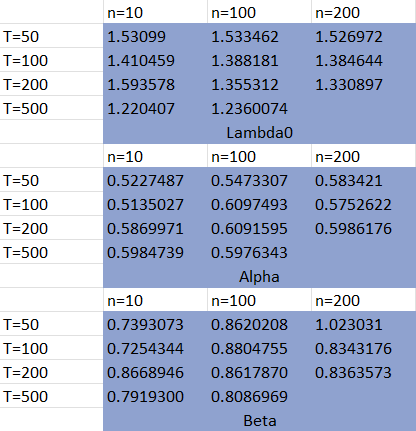
\includegraphics[width=0.5\linewidth]{figures/estim.png}
        \end{figure}
\end{frame}








% La 2e partie: Le point de vue de la relativité restreinte
% Titre de la partie
\section[Pratique]{Application sur la Crimes Database Chicago Police Department}

%%%%%%%%%%%%%%%%%%%%%%%%%%%%%%%%%%%%%%%%%%%%%%%%
% Première diapo (avec des équations)
%%%%%%%%%%%%%%%%%%%%%%%%%%%%%%%%%%%%%%%%%%%%%%%%
\begin{frame}
	\frametitle{Présentation de la base de données}
	\framesubtitle{Chicago Crimes Database 2020}
		\begin{figure}
			    \centering
				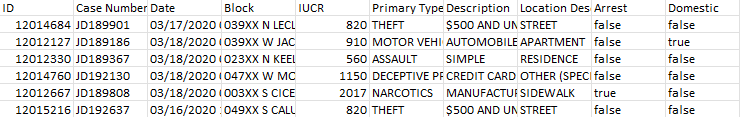
\includegraphics[width=1.0\linewidth]{figures/database.png}
			
		\end{figure}
            \begin{figure}
			    \centering
				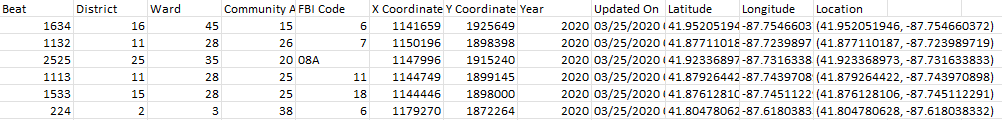
\includegraphics[width=1.0\linewidth]{figures/database2.png}
			
		\end{figure}
\end{frame}

\begin{frame}
	\frametitle{Présentation de la base de données}
	\framesubtitle{Filtrage de la base de données}
 \begin{block}{Filtrage}
    \begin{itemize}
            \item Supprimer les lignes avec des données manquantes
            \item Conserver uniquement les cambriolages
            \item Conserver uniquement les colonnes suivantes : Date, Primary Type, Latitude et Longitude
        \end{itemize}

    \end{block}
\end{frame}

\begin{frame}
	\frametitle{Présentation de la base de données}
	\framesubtitle{Formatage de la base de données}
 \begin{block}{Formatage}
    \begin{itemize}
            \item Passage du format date US au format EU
            \item Trier les cambriolages par ordre chronologique
            \item Définition de l'instant $t_0$=0 correspondant à l'instant du 01/01/2020 à 00H00
        \end{itemize}

    \end{block}
\end{frame}

\begin{frame}
	\frametitle{Présentation de la base de données}
	\framesubtitle{Première analyse}
\begin{alertblock}{Problèmes rencontrés}
\begin{itemize}
            \item Liste trop longue 
            \item Valeurs des instants trop grandes
            \end{itemize}
	\end{alertblock}

 \begin{block}{Solutions exploitées}
 \begin{itemize}
            \item Restriction spatiale
            \item Changement échelle temporelle
            \end{itemize}
	\end{block}
\end{frame}

\begin{frame}
	\frametitle{Présentation de la base de données}
	\framesubtitle{Chicago Crimes Database 2020}
         \begin{block}{Affichage Chicago Map}
		\begin{figure}
			    \centering
				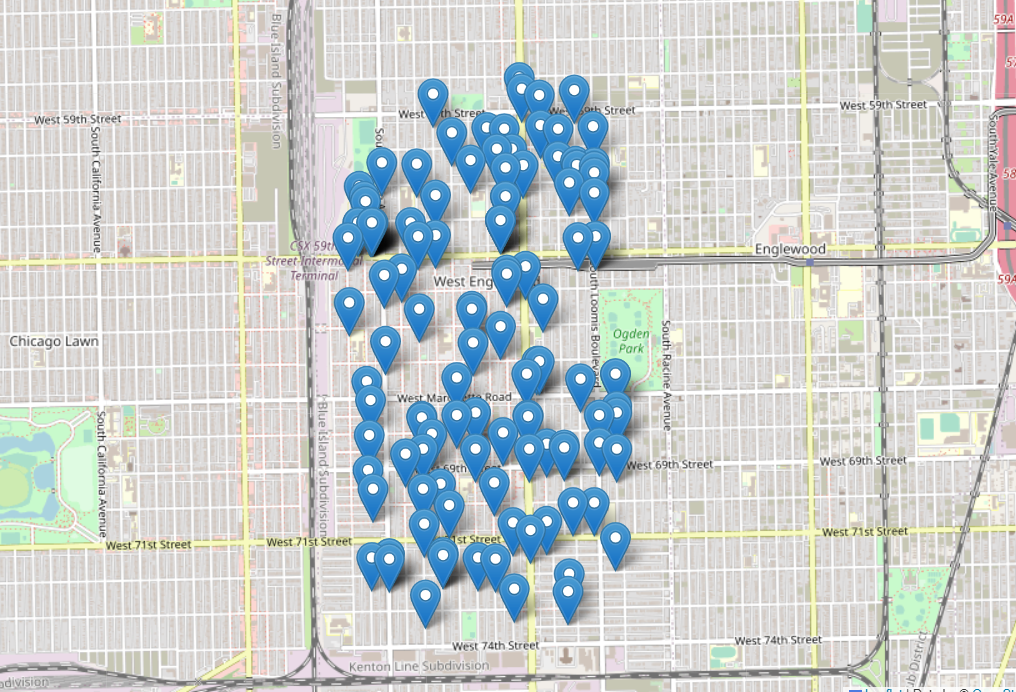
\includegraphics[width=0.8\linewidth]{figures/MAP.png}
			
		\end{figure}
  \end{block}
\end{frame}

\begin{frame}
	\frametitle{Présentation de la base de données}
	\framesubtitle{Premières estimations}
         \begin{block}{Estimations des paramètres}
         \begin{itemize}
            \item $\lambda_0$=0.3067893
            \item $\alpha$=0.11263505
            \item $\beta$=0.03089197
            \end{itemize}
  
  \end{block}

  \begin{block}{Estimations des cambriolages}
         \begin{itemize}
            \item Nombre réel: 125 
            \item Nombre simulé: 125
            \end{itemize}
  
  \end{block}
\end{frame}

\begin{frame}
    \frametitle{Application du modèle}
    \framesubtitle{}
        \begin{figure}
            \centering
            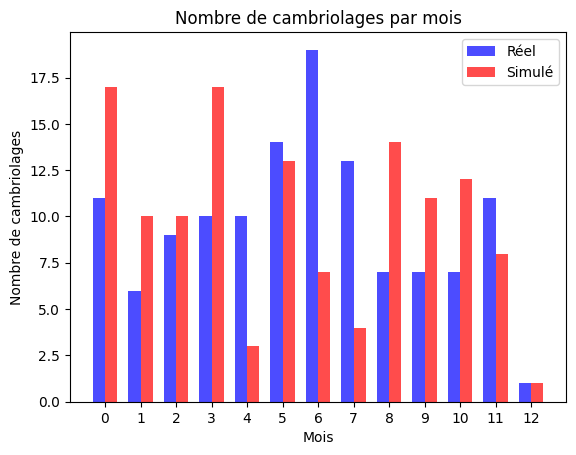
\includegraphics[width=0.6\linewidth]{figures/téléchargement (3).png}
        \end{figure}
\end{frame}

\begin{frame}
    \frametitle{Application du modèle}
    \framesubtitle{Exemple Fonction Calibrage(instants, 50)}
        \begin{figure}
            \centering
            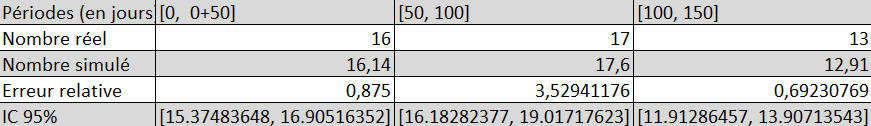
\includegraphics[width=1.0\linewidth]{figures/tab2.png}
        \end{figure}
        \begin{figure}
            \centering
            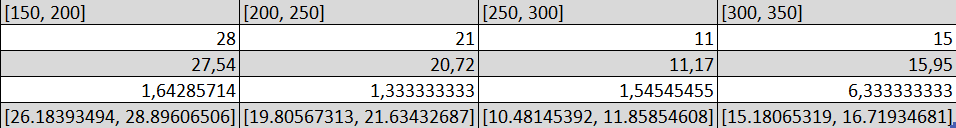
\includegraphics[width=1.0\linewidth]{figures/tab3.png}
        \end{figure}
\end{frame}

\begin{frame}
	\frametitle{Application du modèle}
	\framesubtitle{Calibrage}
         \begin{block}{Estimations des paramètres}
         \begin{itemize}
            \item $\lambda_0$=0.30990218
            \item $\alpha$=0.13504193
            \item $\beta$=0.02762651
            \end{itemize}
  
  \end{block}

    \begin{block}{Estimations des cambriolages}
         \begin{itemize}
            \item Nombre réel: 125 
            \item Nombre simulé: 123
            \end{itemize}
  
  \end{block}
\end{frame}

\begin{frame}
    \frametitle{Application du modèle}
    \framesubtitle{}
        \begin{figure}
            \centering
            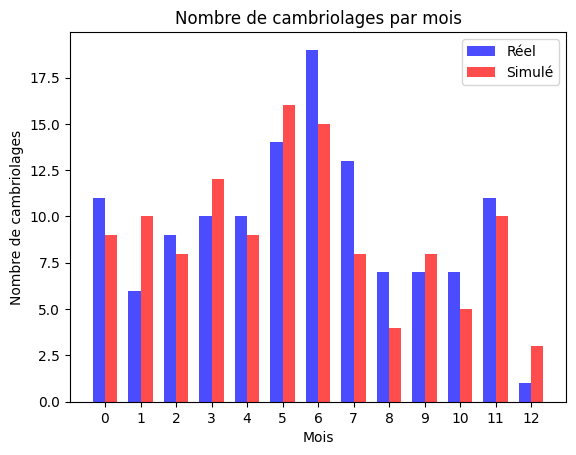
\includegraphics[width=0.6\linewidth]{figures/téléchargement (1).png}
        \end{figure}
\end{frame}



% La 3e partie: Le point de vue de la relativité générale
% Le titre de la partie
\section[Validation]{Tentatives de prédiction des cambriolages dans la ville de Chicago et commentaires}

%%%%%%%%%%%%%%%%%%%%%%%%%%%%%%%%%%%%%%%%%%%%%%%%
% Première diapo (avec des équations)
%%%%%%%%%%%%%%%%%%%%%%%%%%%%%%%%%%%%%%%%%%%%%%%%
\begin{frame}
    \frametitle{Validation du modèle}
    \framesubtitle{}
    \begin{block}{Résultats}
         \begin{itemize}
            \item Correspondance avec les données réelles
            \item Qualité du modèle (erreur relative faible de 2.44\%)
            \item Pertinence du processus de Hawkes
            \item Utilité pour la prévision ?
            \end{itemize}
  
  \end{block}    
\end{frame}

\begin{frame}
    \frametitle{Utilisation du modèle}
    \framesubtitle{Prévisions du nombre de cambriolages en 2021}
    \begin{block}{Résultats}
         \begin{itemize}
            \item Nombre réel: 107 
            \item Nombre prédit: 109
            \end{itemize}
  \end{block}    
\end{frame}

\begin{frame}
    \frametitle{Application du modèle}
    \framesubtitle{}
        \begin{figure}
            \centering
            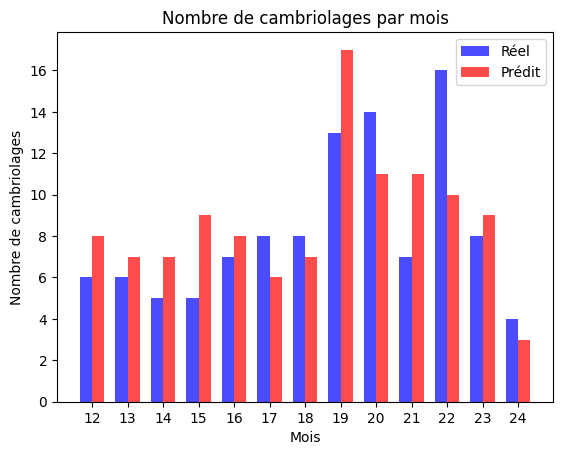
\includegraphics[width=0.6\linewidth]{figures/téléchargement (4).png}
        \end{figure}
\end{frame}

\begin{frame}
    \frametitle{Utilisation du modèle}
    \framesubtitle{Limites du modèle}
    \begin{block}{Limites du modèle}
        \begin{itemize}
            \item Simplification du processus réel
            \item Hypothèses du modèle
            \item Prédictions à long terme
            \item Sensibilité aux paramètres
            \item Difficulté de calibrage
            \item Manque d'explications causales 
        \end{itemize}
    \end{block}    
\end{frame}


\begin{frame}
    \frametitle{Utilisation du modèle}
    \framesubtitle{Limites du modèle}
    \begin{alertblock}{Peut-on envisager l'utilisation d'un tel modèle dans la vie courante? L'exemple de PredPol}
        \begin{figure}
            \centering
            
\includegraphics[width=0.6\linewidth]{figures/CorteX_predpol_slogan.jpg}
            \caption{www.predpol.com}
        \end{figure}
    \end{alertblock}
\end{frame}

\begin{frame}
    \frametitle{Utilisation du modèle}
    \framesubtitle{Limites du modèle}
    \begin{alertblock}{Peut-on envisager l'utilisation d'un tel modèle dans la vie courante? L'exemple de PredPol}
        \begin{figure}
            \centering
            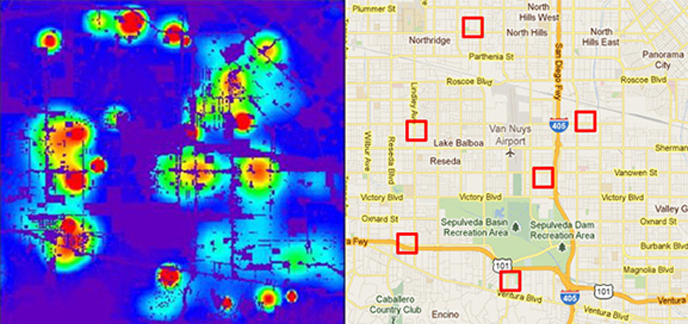
\includegraphics[width=0.6\linewidth]{figures/i_predpol.jpg}
            \caption{www.predpol.com}
        \end{figure}
    \end{alertblock}
\end{frame}

\begin{frame}
    \frametitle{Fin du TIPE}
    \framesubtitle{}
        \centering
        \Large{Merci pour votre attention!}
\end{frame}





\appendix
%%%%%%%%%%%%%%%%%%%%%%%%%%%%%%%%%%%%%%%%%%%%%%%%
% Le code informatique impose un
% environnement "fragile" pour la frame
%%%%%%%%%%%%%%%%%%%%%%%%%%%%%%%%%%%%%%%%%%%%%%%%
\section[Annexe]{}


\begin{frame}[allowframebreaks]
    \frametitle{Annexe}
    \framesubtitle{Code Python}
    \lstinputlisting[basicstyle=\fontsize{1}{1}\ttfamily, language=Python]{Annexe.py}
\end{frame}





\end{document}
